\section{Flaches tiefes neuronales Netz zur Klassifizierung von OCT Aufnahmen der Retina}

Um die Wahl des CNN zu validieren wird diese mit einer alternativen Methode verglichen. Diese basiert auf einem falchen tiefen neuronalen Netz (DNN), welches aus vollständig vernetzten dichten Lagen besteht. \\
Hierzu müssen die analysierten Bilder zunächst in eine 1 dimensionale Liste aus Werten umgewandelt werden. Hierzu muss beachtet werden, dass diese Liste nicht zu groß werden darf, da ansonsten das Training und die Optimierung des neuronalen Netzes zu zeitaufwendig ist. Demnach wird die Dimension der Aufnahmen zunächst auf $(50\times 100)$ reduziert.\\
Darauf aufbauend werden drei Verfahren untersucht aus diesen Bilder eine 1 dimensionale Liste zu erstellen, welche als Eingangseigenschaften des DNN der Aufnahmen verwendet werden. Zum einen werden alle Pixelwerte einer $(50\times 100)$ Aufnahme in eine 1 dimensionale Liste umgewandelt und dem DNN übergeben. Erste Studien hierzu liefern eine Genauigkeit der Klassifikation von ungefähr $55\,\%$. Die zweite Methode basiert darauf für jede $x$- und $y$-Linie des Aufnahme den Mittelwert aller Pixelwerte der jeweiligen Linie zu berechnen. Demnach generiert sich eine Liste aus 150 Werten. Die Werte werden dabei auf den maximalen Wert dieser List skaliert. Auch bei dieser Methodik wird eine Genauigkeit von ungefähr $55\,\%$ erzielt. Die letzte Methode basiert darauf das Bild weiter zu verkleinern, indem ein Fenster der Dimension $(2\times 4)$ definiert wird, welches die Aufnahmen abrastert. Dabei soll keine Überlappung der einzelnen Schritte entstehen. Der Mittelwert der im Fenster liegenden Pixel wird für jeden Schritt der Abrasterung berechnet. Anschließend werden die so erhaltenen Mittelwerte auf den größten Mittelwert einer Aufnahme skaliert und dem DNN übergeben. In den vereinfachten ersten Studien zeigte sich bei dieser Methode eine Genauigkeit von $70\,\%$, wodurch diese vielversprechend erscheint und im Folgenden betrachtet wird. \\
% Abbildung \ref{fig:input} zeigt beispielhaft für jede der Klassen das $(50,\,100)$ Bild sowie die aus dem resultierende Verteilung der Mittelwerte. Die gewählten Beispiele sind so ausgewählt worden, dass anhand der Aufnahmen bereits per Auge eine Entscheidung getroffen werden kann, sodass dies den Fall representiert bei dem eine Klassifizierung der Bilder sehr gut möglich ist. Das ist jedoch nicht bei allen  Bildern der Fall. Ein Blick auf die Verteilungen der Mittelwerte lässt bereits den Schluss zu, dass CNV die Klasse darstellt, die am besten von den anderen zu trennen ist. Es ist außerdem zu erwarten, dass sich DRUSEN von NORMAL schwer unterscheiden lässt. \\
Um eine geeignete Referenzstruktur des DNN zu finden mit der das CNN verglichen werden kann, werden verschiedene Netzstrukturen ausprobiert. Es werden 5 Grundstrukturen des DNN definiert, welche in Tabelle \ref{tab:DNNstruk} dargestellt sind und als Modell $i$ ($i = 0,\,1,\,2,\,3,\,4$) bezeichnet werden. Dabei folgt auf jede versteckte Lage eine Dropout Lage, wobei die Anzahl an Ausgangsknoten und verwendeten Dropout-Rate der $i$-ten Lage durch das $i$-te Element in den entsprechenden Listen daragestellt ist. \\
\begin{table}[!b]
\centering
\caption{Getestete Grundstrukturen des DNN.}
\label{tab:DNNstruk}
 \begin{tabular}{c|c|c}
 & Struktur der versteckten dichten Lagen & Struktur der Dropout Lagen \\
 \hline
 Modell 0 & (1024, 512, 128, 64, 32) & (0.5, 0.4, 0.4, 0.3, 0.2) \\
 Modell 1 & (1024, 512, 256, 128, 64, 32, 16) & (0.5, 0.4, 0.4, 0.4, 0.2, 0.2, 0.1)\\
 Modell 2 & (512, 256, 128, 64, 32, 16) & (0.4, 0.4, 0.3, 0.3, 0.2, 0.1)\\
 Modell 3 & (1024, 256, 64, 16) & (0.6, 0.4, 0.2, 0.1)\\
 Modell 4 & (512, 128, 32) &  (0.5, 0.3, 0.1)\\
 \end{tabular}
\end{table}
Für jede der fünf Grundstrukturen werden die Aktivierungsfunktionen elu und relu für die versteckten Lagen und die Aktivierungsfunktionen softmax und sigmoid für die Ausgangslage variiert. Zudem werden die Batch Größen 50, 100, 128, 256 und 512 für jede der sich ergebenden DNN Konfigurationen getestet. Insgesamt werden somit 120 Konfigurationen für das Training des DNN getestet. \\
Als Verlustfunktion wird wie beim CNN die kategorische Kreuzentropie verwendet und als Metrik die Genauigkeit betrachtet. Der Adam Optimierer wird auch hierbei mit einer angepassten Lernrate von 0.0001 benutzt. Der Datensatz wird in den Trainings-, Validierungs- und Testdatensatz aufgeteilt, die aus $67,5\,\%$, $25\,\%$ und $7,5\,\%$ des kompletten Datensatzes bestehen. Die verschiedenen Konfigurationen werden jeweils 150 Epochen lang trainiert. Die Werte der Genauigkeit bei Propagation des Validierungsdatensatzes als Funktion der Batch Größe ist für jede Konfiguration eines Modells in Abbildung \ref{fig:accgrid} dargestellt.\\
\begin{figure}[!t]
 \centering
\begin{subfigure}[Modell 0]{
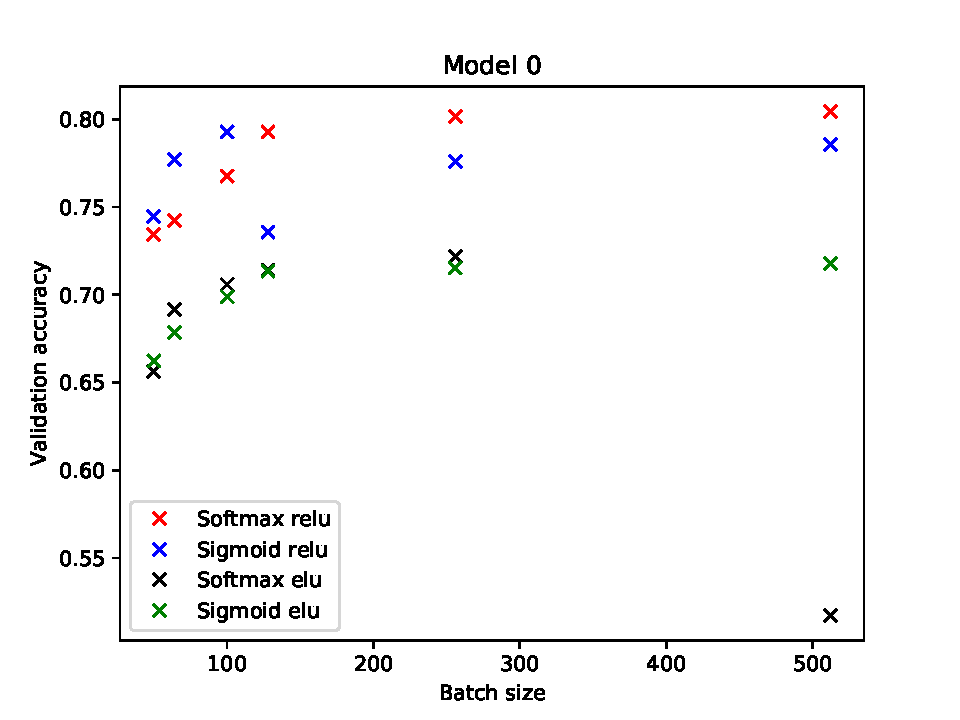
\includegraphics[width=.30\linewidth]{fig/Modelvalacc0.pdf}}
\end{subfigure}%
\begin{subfigure}[Modell 1]{
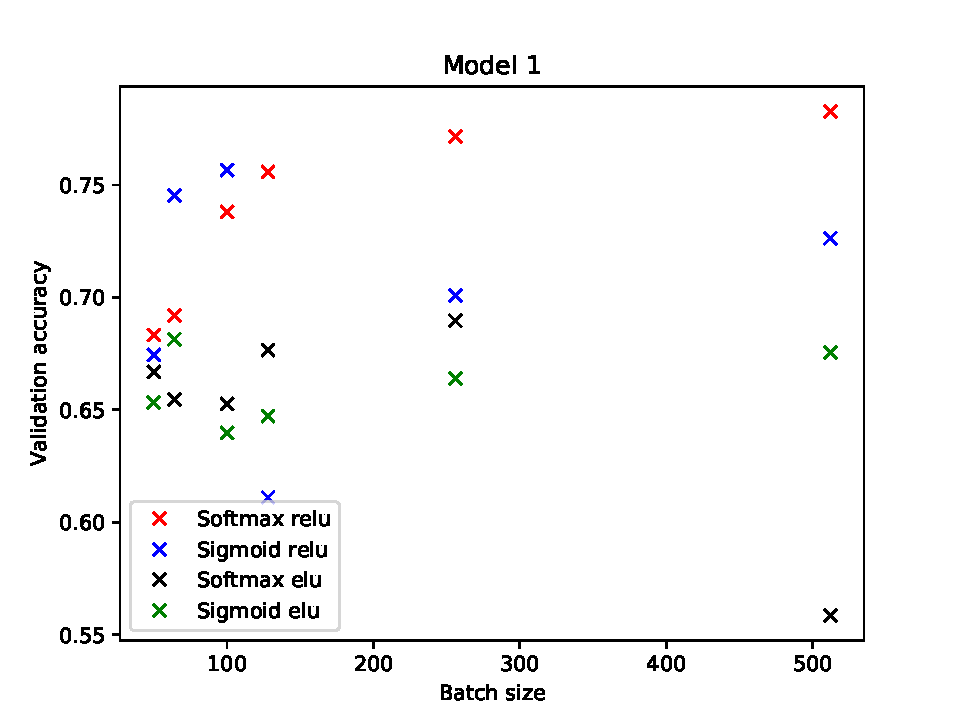
\includegraphics[width=.30\linewidth]{fig/Modelvalacc1.pdf}}
\end{subfigure}
\begin{subfigure}[Modell 2]{
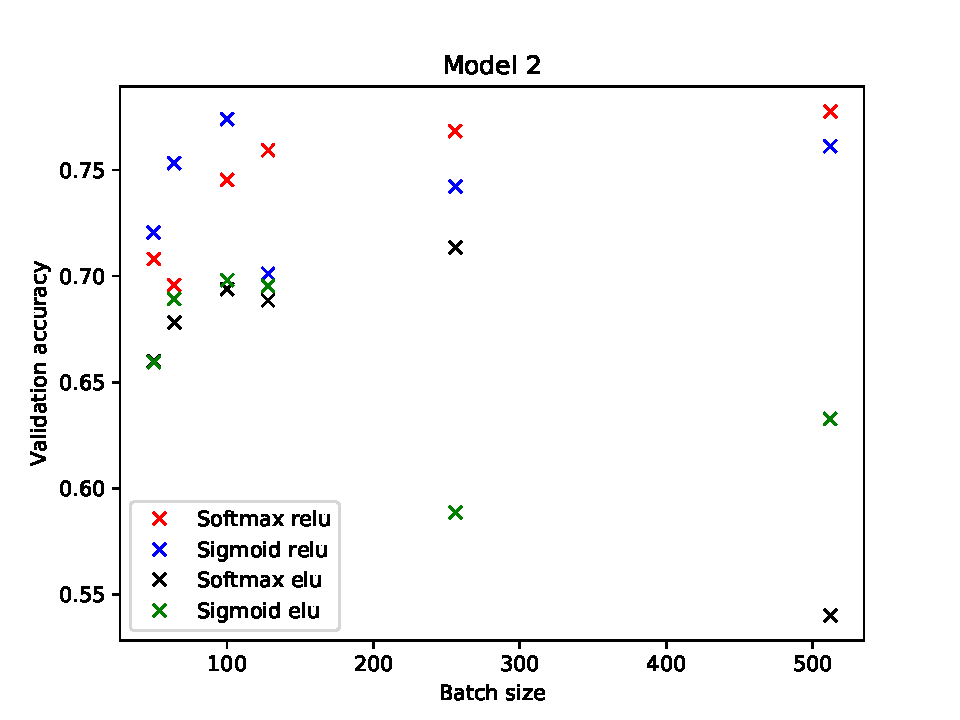
\includegraphics[width=.30\linewidth]{fig/Modelvalacc2.pdf}}
\end{subfigure}\\
\begin{subfigure}[Modell 3]{
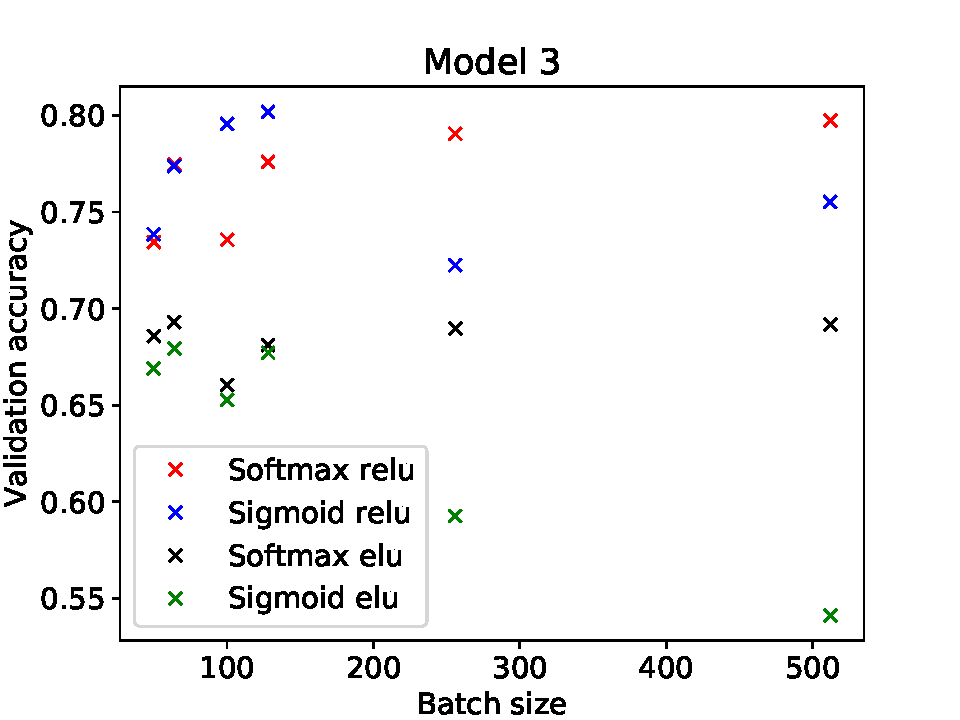
\includegraphics[width=.30\linewidth]{fig/Modelvalacc3.pdf}}
\end{subfigure}
\begin{subfigure}[Modell 4]{
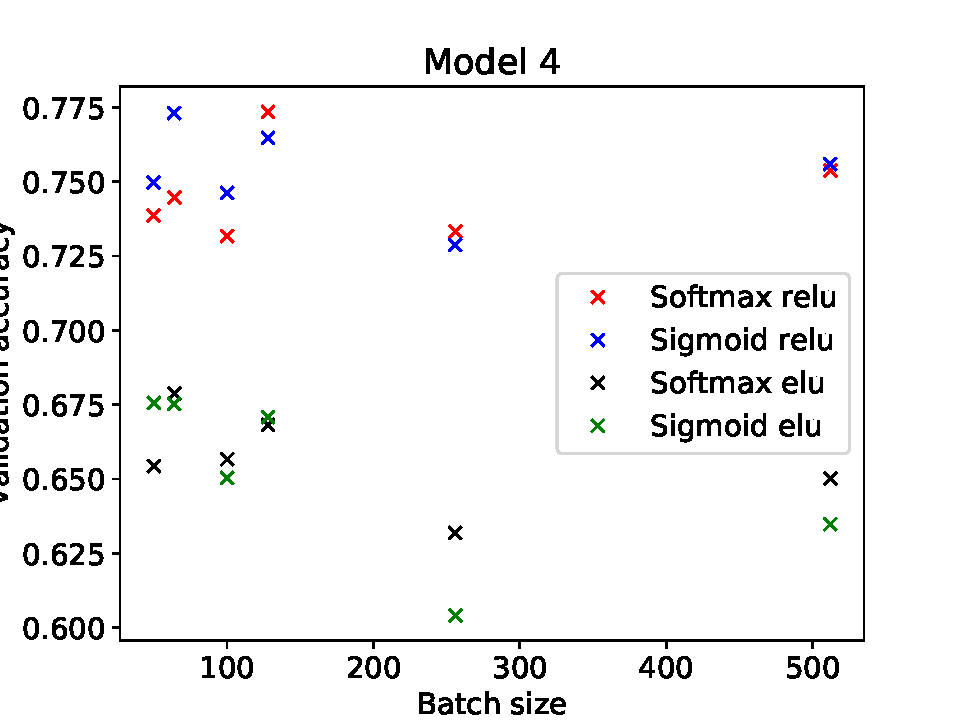
\includegraphics[width=.30\linewidth]{fig/Modelvalacc4.pdf}}
\end{subfigure}
\caption{Erhaltene Genauigkeiten des DNN für die verschiedenen Konfigurationen der einzelnen Modelle als Funktion der Batch Größe.}
\label{fig:accgrid}
\end{figure}
\setcounter{subfigure}{0}
Um ungeeignete DNN Konfigurationen herauszufiltern werden zwei verschiedene Kriterien definiert, die von den Konfigurationen erfüllt werden müssen. Zum einen muss die Genauigkeit auf dem Validierungsdatensatz größer als $73\,\%$ sein. Das zweite Kriterium filtert Konfigurationen heraus, die ein starkes Übertraining aufweisen, indem gefordert wird, dass der Wert der Verlustfunktion nach der ersten Epoche um mindestens $5\,\%$ nach der letzten Epoche gesunken ist. Nach diesen Anwendung dieser Selektionskriterien verbleiben 12 DNN Konfigurationen. Es stellt sich hierbei vor allem heraus, dass hohe Batch Größen ungeeignet sind, da keine der Konfigurationen mit einer Batch Größe von 512 und nur eine Konfiguration mit einer Batch Größe von 256 die Selektionsschritte passieren. Um nun die optimale herauszufiltern, wird die Gesamtgenauigkeit wie im Falle des CNN berechnet und das Maximum gesucht. Dieses ergibt sich für das Modell 0 unter Verwendung der relu Funktion als Aktivierungsfunktion der versteckten Lagen und der sigmoid Funktion als Aktivierungsfunktion der Ausgangslage bei einer Batch Größe von 50 und beträgt $72\,\%$ auf dem Validierungsdatensatz. Der Verlauf der Genauigkeit und der Werte der Verlustfunktion sind als Funktion der Epochen in Abbildung \ref{fig:DNNacc} respektive \ref{fig:DNNloss} dargestellt. \\
\begin{figure}[!t]
\centering
 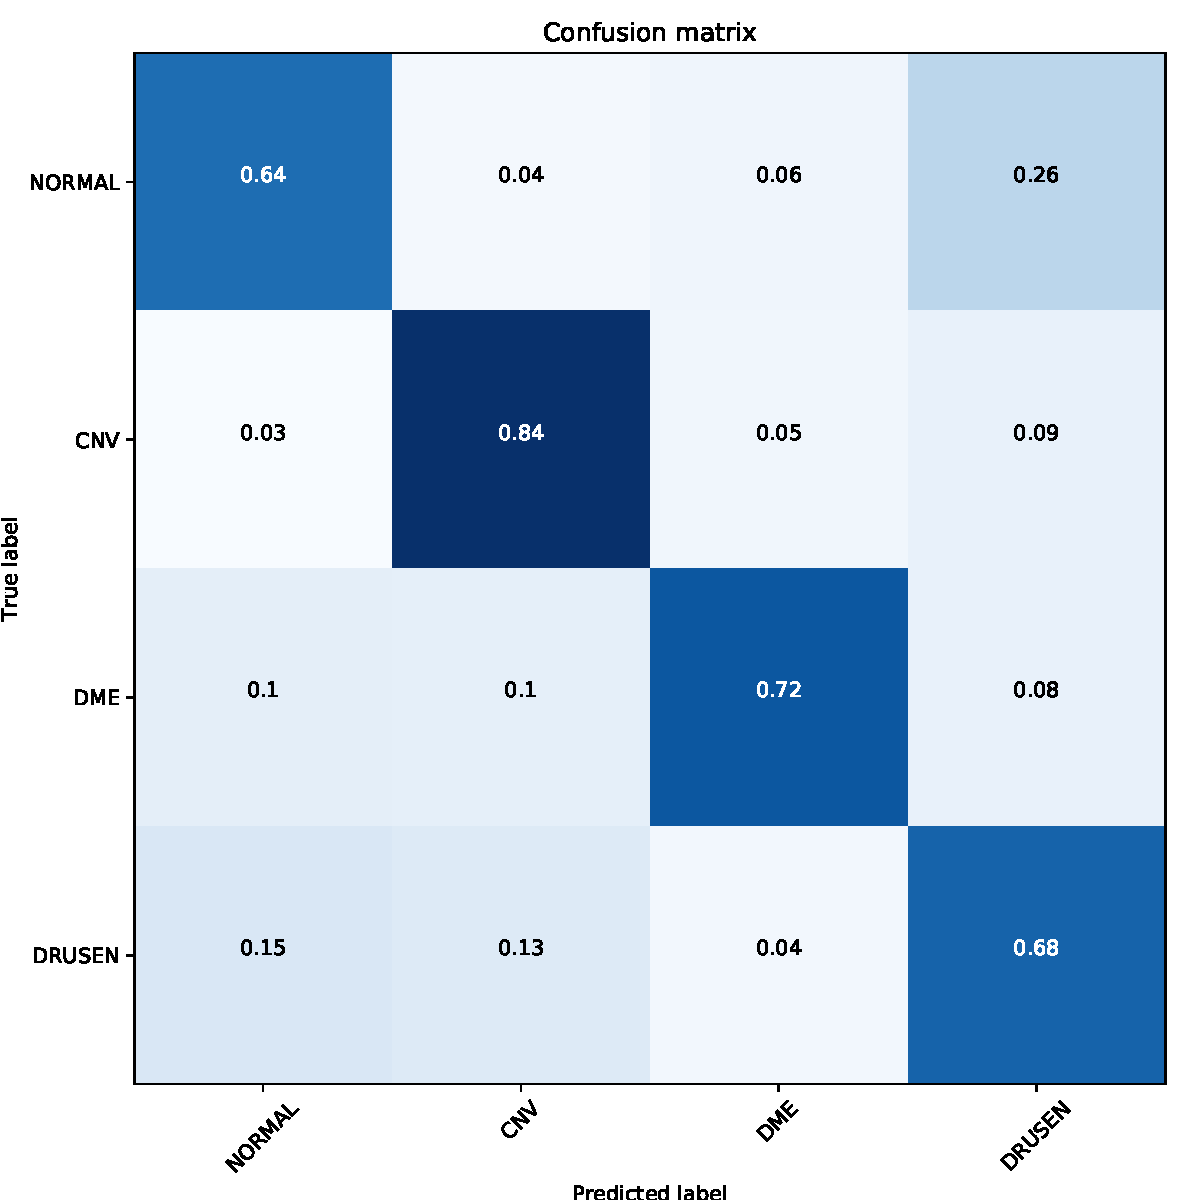
\includegraphics[width=.55\linewidth]{fig/confusionmatrix6test.pdf}
 \caption{Verwirrungsmatrix der gewählten DNN Konfiguration ermittelt auf dem Trainingsdatensatz.}
 \label{fig:ConfmatDNN}
\end{figure}
Anhand \ref{fig:DNN} lässt sich zudem feststellen, dass kein signifikantes Übertraining vorhanden ist und die Genauigkeit bereits einen Sättigungswert erreicht hat. In Abbildung \ref{fig:ConfmatDNN} ist die entsprechende Verwirrungsmatrix dargestellt, welche auf dem Trainingsdatensatz ermittelt wird. Auch hier errechnet sich eine Gesamtgenauigkeit von $72\,\%$, wodurch bestätigt wird, dass das DNN eine geeignete Struktur aufweist, die kein starkes Übertraining besitzt. 
\begin{figure}[!b]
 \centering
   \begin{subfigure}[Genauigkeit]{
 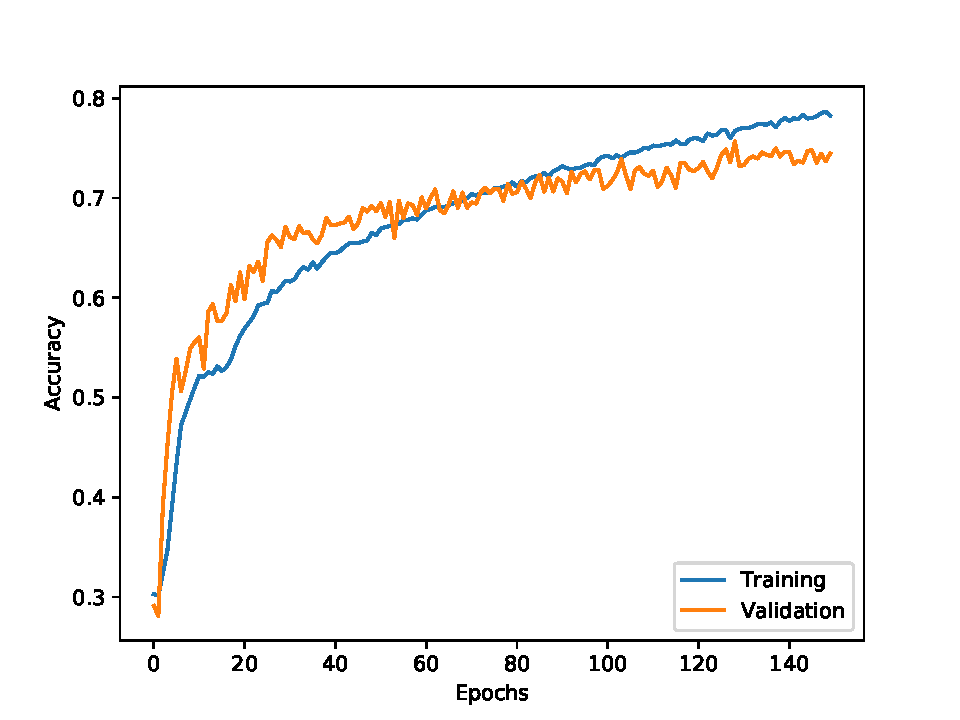
\includegraphics[width=.45\linewidth]{fig/accuracyhistory6.pdf}\label{fig:DNNacc}}
  \end{subfigure}
 \begin{subfigure}[Verlustfunktion]{
 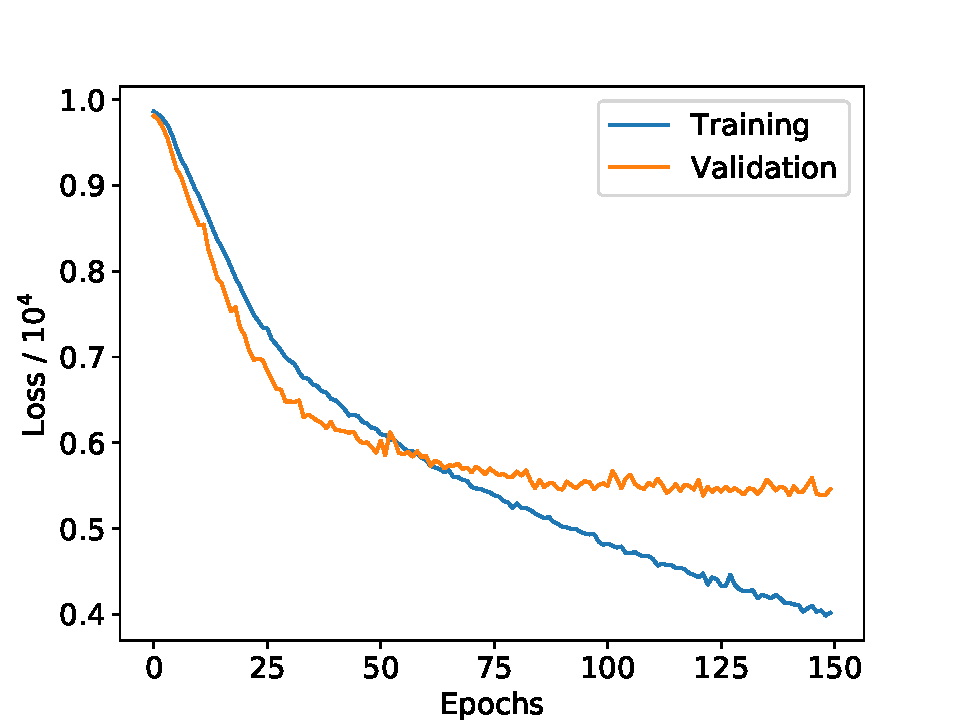
\includegraphics[width=.45\linewidth]{fig/losshistory6.pdf}\label{fig:DNNloss}}
  \end{subfigure}
  \caption{Genauigkeit und Wert der Verlustfunktion für die gewählte DNN Struktur als Funktion der Epoche bei Propagation des Trainings- und Validierungsdatensatzes. }
  \label{fig:DNN}
\end{figure}
\setcounter{subfigure}{0}












